

\subsubsection{Sintassi di Base}

\paragraph{Creazione di Liste}

In Python, esistono diversi modi per creare una lista. Ecco i metodi più comuni:

\begin{lstlisting}[language=Python]
# Lista vuota
lista_vuota = []

# Lista di numeri
numeri = [1, 2, 3, 4, 5]

# Lista di stringhe
nomi = ["Anna", "Bruno", "Carlo", "Daria"]

# Lista con elementi di tipi diversi
lista_mista = [1, "Python", 3.14, True]

# Lista nidificata (liste all'interno di liste)
matrice = [[1, 2, 3], [4, 5, 6], [7, 8, 9]]

# Creazione di lista mediante la funzione list()
caratteri = list("Python")  # Crea la lista ['P', 'y', 't', 'h', 'o', 'n']
numeri_sequenza = list(range(1, 6))  # Crea la lista [1, 2, 3, 4, 5]
\end{lstlisting}

\begin{nota}
La funzione \texttt{list()} può convertire in lista qualsiasi oggetto che sia \textit{iterabile} (ovvero che possa essere percorso elemento per elemento). Nel secondo esempio, \texttt{range(1, 6)} crea una sequenza di numeri da 1 a 5, che viene convertita in lista.
\end{nota}

\paragraph{Best Practice per Denominare le Liste}

Una buona denominazione delle variabili è fondamentale per la leggibilità del codice. Per le liste, seguire queste linee guida può rendere il codice più comprensibile:
come già affrontato per le variabili, breve ripasso;\textit{\nameref{bestPractice}}

\begin{tcolorbox}[colback=green!5!white,colframe=green!75!black,title=Best practice per i nomi delle liste]
\begin{itemize}
    \item \textbf{Usa nomi al plurale}: Poiché le liste contengono tipicamente più elementi, è consigliabile usare nomi plurali (es. \texttt{studenti} anziché \texttt{studente})
    
    \item \textbf{Scegli nomi descrittivi}: Il nome dovrebbe suggerire cosa contiene la lista
    \begin{itemize}
        \item Buono: \texttt{prezzi\_prodotti}, \texttt{nomi\_studenti}, \texttt{temperature\_giornaliere}
        \item Da evitare: \texttt{l}, \texttt{lista1}, \texttt{dati}, \texttt{cose}
    \end{itemize}
    
    \item \textbf{Segui le convenzioni Python}: Usa \texttt{snake\_case} (parole in minuscolo separate da underscore)
    
    \item \textbf{Coerenza nei tipi}: Se la lista contiene elementi dello stesso tipo, considera di indicarlo nel nome (es. \texttt{numeri\_pari}, \texttt{stringhe\_input})
\end{itemize}
\end{tcolorbox}

\begin{esempio}
Confronto tra nomi poco chiari e nomi appropriati:

\begin{tabular}{|l|l|l|}
\hline
\textbf{Nome sconsigliato} & \textbf{Nome consigliato} & \textbf{Contenuto} \\
\hline
\texttt{l} o \texttt{lst} & \texttt{studenti} & Lista di nomi di studenti \\
\texttt{nums} & \texttt{voti\_esame} & Lista di voti numerici \\
\texttt{x} & \texttt{coordinate\_x} & Lista di valori delle coordinate x \\
\texttt{lista\_dati} & \texttt{temperature\_mensili} & Lista di temperature \\
\hline
\end{tabular}
\end{esempio}

\subsubsection{Accesso agli Elementi}\label{AccessoListe}

Per accedere a un elemento specifico di una lista, si utilizzano gli indici racchiusi tra parentesi quadre:

\begin{lstlisting}[language=Python]
colori = ["rosso", "verde", "blu", "giallo", "viola"]

# Accesso al primo elemento (indice 0)
primo_colore = colori[0]  # "rosso"

# Accesso al terzo elemento (indice 2)
terzo_colore = colori[2]  # "blu"

# Accesso all'ultimo elemento (indice -1)
ultimo_colore = colori[-1]  # "viola"

# Accesso al penultimo elemento (indice -2)
penultimo_colore = colori[-2]  # "giallo"
\end{lstlisting}

\begin{attenzione}
Se si tenta di accedere a un indice che non esiste, Python genererà un errore \texttt{IndexError}. Ad esempio, \texttt{colori[10]} genererà un errore se la lista \texttt{colori} ha meno di 11 elementi.
\end{attenzione}

\subsubsection{Modifica degli Elementi}\label{ModificaEleListe}

Essendo le liste mutabili, è possibile modificare i singoli elementi assegnando nuovi valori:

\begin{lstlisting}[language=Python]
# Lista iniziale
frutta = ["mela", "banana", "pera", "arancia"]

# Modifica del secondo elemento
frutta[1] = "kiwi"
# Ora frutta e' ["mela", "kiwi", "pera", "arancia"]

# Modifica dell'ultimo elemento usando indice negativo
frutta[-1] = "limone"
# Ora frutta è ["mela", "kiwi", "pera", "limone"]
\end{lstlisting}

È anche possibile modificare più elementi contemporaneamente utilizzando lo slicing:

\begin{lstlisting}[language=Python]
numeri = [1, 2, 3, 4, 5]

# Sostituzione di più elementi
numeri[1:4] = [20, 30, 40]
# Ora numeri è [1, 20, 30, 40, 5]

# Si può anche sostituire con un numero diverso di elementi
numeri[1:4] = [200, 300]
# Ora numeri è [1, 200, 300, 5]
\end{lstlisting}

\subsubsection{Slicing di Liste}\label{SlicingListe}

Lo slicing permette di estrarre una porzione di una lista, creando una nuova lista. La sintassi generale è \texttt{lista[inizio:fine:passo]}, dove:
\begin{itemize}
    \item \texttt{inizio} è l'indice da cui iniziare (incluso)
    \item \texttt{fine} è l'indice dove terminare (escluso)
    \item \texttt{passo} è il passo con cui avanzare (opzionale, default 1)
\end{itemize}

\begin{lstlisting}[language=Python]
numeri = [0, 1, 2, 3, 4, 5, 6, 7, 8, 9]

# Elementi dal secondo al quarto (indici 1, 2, 3)
sottosequenza = numeri[1:4]  # [1, 2, 3]

# Primi tre elementi
inizio = numeri[:3]  # [0, 1, 2]

# Elementi dal quarto fino alla fine
fine = numeri[3:]  # [3, 4, 5, 6, 7, 8, 9]

# Ultimi tre elementi
ultimi = numeri[-3:]  # [7, 8, 9]

# Tutti gli elementi tranne gli ultimi due
senza_ultimi = numeri[:-2]  # [0, 1, 2, 3, 4, 5, 6, 7]

# Elementi con indici pari (passo 2)
pari = numeri[::2]  # [0, 2, 4, 6, 8]

# Elementi in ordine inverso
inverso = numeri[::-1]  # [9, 8, 7, 6, 5, 4, 3, 2, 1, 0]
\end{lstlisting}

\begin{center}
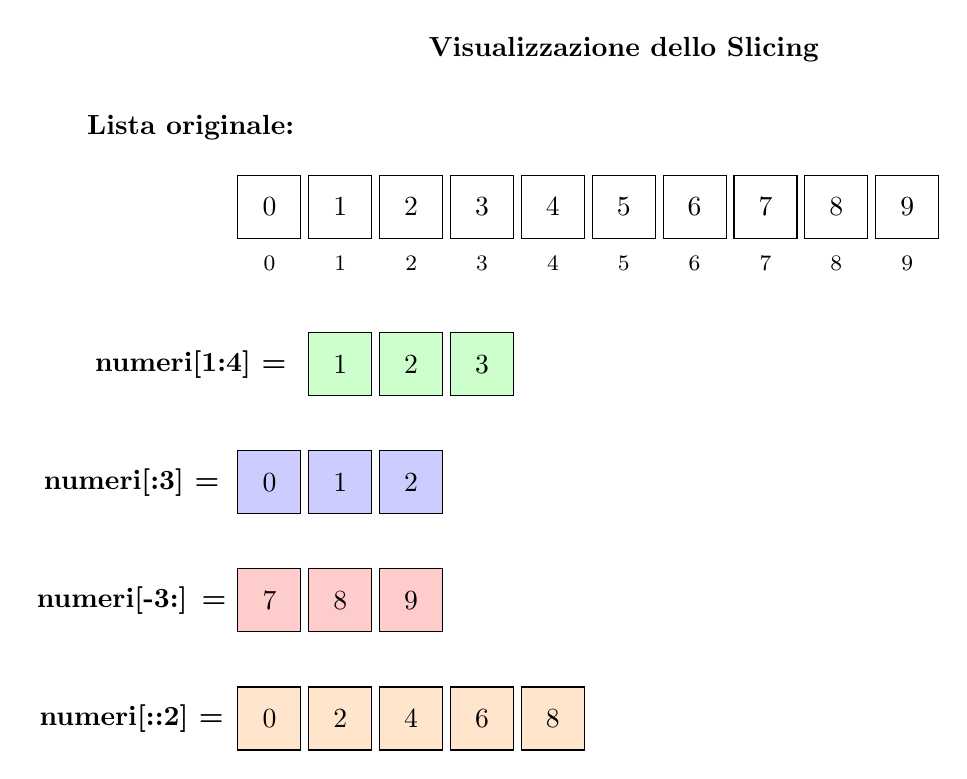
\begin{tikzpicture}
    % Titolo
\node[font=\bfseries] at (0,2) {Visualizzazione dello Slicing};
% Lista originale
\node[font=\bfseries] at (-5.5,1) {Lista originale:};
\foreach \x [count=\i from 0] in {0,1,2,3,4,5,6,7,8,9} {
    \node[draw, minimum width=0.8cm, minimum height=0.8cm] at (\i*0.9-4.5,0) {\x};
    \node[below] at (\i*0.9-4.5,-0.5) {\footnotesize\i};
}

% Esempi di slicing
\begin{scope}[yshift=-2cm]
    \node[font=\bfseries, align=right] at (-5.5,0) {numeri[1:4] =};
    \foreach \x [count=\i from 1] in {1,2,3} {
        \node[draw, fill=green!20, minimum width=0.8cm, minimum height=0.8cm] at (\i*0.9-4.5,0) {\x};
    }
\end{scope}

\begin{scope}[yshift=-3.5cm]
    \node[font=\bfseries, align=right] at (-5.5,0) {numeri[:3] =\hspace{1.5cm}}; 
    \foreach \x [count=\i from 0] in {0,1,2} {
        \node[draw, fill=blue!20, minimum width=0.8cm, minimum height=0.8cm] at (\i*0.9-4.5,0) {\x};
    }
\end{scope}

\begin{scope}[yshift=-5cm]
    \node[font=\bfseries, align=right] at (-5.5,0) {numeri[-3:] =\hspace{1.5cm}}; 
    \foreach \x [count=\i from 0] in {7,8,9} {
        \node[draw, fill=red!20, minimum width=0.8cm, minimum height=0.8cm] at (\i*0.9-4.5,0) {\x};
    }
\end{scope}

\begin{scope}[yshift=-6.5cm]
    \node[font=\bfseries, align=right] at (-5.5,0) {numeri[::2] =\hspace{1.5cm}};
    \foreach \x [count=\i from 0] in {0,2,4,6,8} {
        \node[draw, fill=orange!20, minimum width=0.8cm, minimum height=0.8cm] at (\i*0.9-4.5,0) {\x};
    }
\end{scope}

\end{tikzpicture}
\end{center}

\begin{nota}
Lo slicing crea sempre una nuova lista, non modifica quella originale. Se vuoi modificare la lista originale, devi effettuare un'assegnazione esplicita (es. \texttt{lista = lista[1:4]}).
\end{nota}